\epi{\lstinline{fmt.Printf("\%p", i)}}{Printing the address of a pointer in Go.}
\noindent

\subsection{Nil value}
A reference to nothing is represented in Go as \lstinline{nil}. This is
different than a zero value. \todo{nil only for references?}

\begin{lstlisting}
var *a int
a = nil
fmt.Printf("%v\n", a);
\end{lstlisting}
Prints \lstinline{nil}.


\section{Arrays, slices and maps}
From \cite{go_intro} ... really Good
%
arrays, even if it doesn't have any other parametric types? And we really want
these cool things called slices - but they really need to be strongly typed. So
we'll let them be parametric. And maps - we really need a map type, which maps
keys to values, and it really needs to be type-safe. So we'll add a parametric
map type to the language, by making it a special case built-in.

So: you can't write parametric types - but they can. And that creates a very
weird asymmetry to the language. Everything in Go is passed by value - except
for the built-in slice and map types, which are passed by reference. Everything
is allocated by "new" - except for the built-in slice and map types, which are
allocated by "make". It's by far the biggest blemish in Go, and it's absolutely
infuriating.

\subsection{Arrays}
Array types like \lstinline{[10]int} have a fixed size.
It can't grow, because then it would have a different type. Also arrays
are values: Assigning one array to another \emph{copies} all the elements.

In particular, if you pass an array to a function, it will receive a
copy of the array, not a pointer to it. This is a major difference with C.

To declare an array you can use the following: \lstinline{var a [3]int},
to initialize it to something else than zero, use a composite literal.
\gomarginindex{composite literals}{composite literals}\lstinline|a := [3]int{1, 2, 3}| and
this can be shortend to \lstinline|a := []int{1, 2, 3}|, where Go counts
the elements automatically.

Note that all fields must be specified.  So if you are using multidimentional
arrays you have to do quite some typing:
\begin{lstlisting}
a := [2][2]int{ [2]int{1,2}, [2]int{3,4} }
\end{lstlisting}
Which is \emph{not} the same as:
\begin{lstlisting}
a := [2][2]int{ []int{1,2}, []int{3,4} }
\end{lstlisting}
As this gives a compile error.\todo{why?}\newline
\lstinline{cannot use slice literal (type []int) as type [2]int in array index}

But this is then OK again:
\begin{lstlisting}
a := [][]int{ []int{1,2}, []int{3,4} }
\end{lstlisting}
So either specify the length of the array or let Go do the counting, but
don't mix the two.
\subsection{Slices}
Slices are reference types, which means that if you assign one slice to
another, both refer to the same underlying array. For instance, if a
function takes a slice argument, changes it makes to the elements of the
slice will be visible to the caller, analogous to passing a pointer to
the underlying array. A slice is always coupled to an array that has
a fixed size. For slices we define a capacity and a length.

\begin{figure}[!bh]
\caption{Array versus slice}
\label{fig:array-vs-slice}
\begin{center}
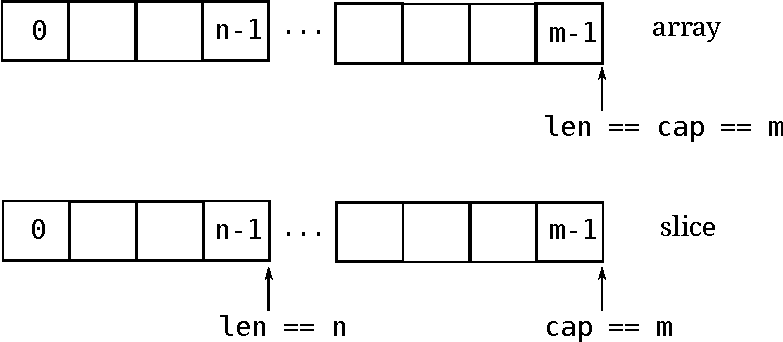
\includegraphics[scale=0.65]{fig/array-vs-slice.pdf}
\end{center}
\end{figure}
Figure \ref{fig:array-vs-slice} depicts the following Go code.
First we create an array of $m$ elements of the type \lstinline{int}:
\lstinline{var array[m + 1]int}\newline
Next, we create a slice from this array:
\lstinline{slice := array[0:n +1]}\newline
And now we have:
\begin{itemize}
\item{\lstinline{len(slice) = n, cap(slice) = m};}
\item{\lstinline{len(array) = cap(array) = m}.}
\end{itemize}
Also see the following code:
\lstinputlisting[numbers=right,label=src:arrays,caption=Arrays and slices]{src/array-and-slices.go}
On line 8 we dare to do to impossible and try to allocate something
behind the capacity (maximum length of the under laying array) and
we are greeted with a \emph{runtime} error

\noindent\lstinline{throw: index out of range}.

\subsection{Maps}
\label{sec:maps}

\section{Conversions}
\label{sec:conversions}
Sometimes you want to convert a type to another type. In C this is known
as casting a value to another type. This is also possible in Go, but
there are some rules.\todo{there are more rules, but we're trying to
keep it simple...}
You can convert:
\begin{itemize}
\item{
From a \lstinline{string} to a slice of \lstinline{byte}s.
\begin{lstlisting}
mystring = "hello this is string"
byteslice =  []byte(mystring)
\end{lstlisting}
}
\item{
From a slice of \lstinline{byte}s to a \lstinline{string}.
\begin{lstlisting}
The other way around
\end{lstlisting}
}
\end{itemize}
\todo{Maybe put this to the end of this chapter}
%%x is an integer or has type []byte or []int and T is a string type.
%%and back
%% integer/float truncation














You may have wished otherwise, but Go has pointers.
There is however now pointer arithmetic and they are still useful.
Remember Go when you call a function in Go the variables you pass are
pass-by-value. So, for efficiency and the possibility to modify a
passed value \emph{in} the function we have pointers.

%% Do we need a whole chapter on Pointers in Go
Just like in C you declare a pointer by prefixing the type with an `*`,
so:

are declared after variable names, and all type modifiers precede the
\todo{}%
types. So *X is a pointer to an X; [3]X is an array of three X's. The
types are therefore really easy to read just read out the names of the
type modifiers: [] declares something called an array slice; "*"
declares a pointer; [size] declares an array. So []*[3]*int is an array
slice of pointers to arrays of three pointers to ints

\noindent\lstinline{var pint *int   // declare pint to be pointer to int}

Note that it's perfectly OK to return the address of a local variable; the
storage associated with the variable survives after the function returns. In
fact, taking the address of a composite literal allocates a fresh instance each
time it is evaluated, so we can combine these last two lines. \cite{effective_go}

\section{Allocation}
Go has garbage collection, meaning that you don't have to worry about
memory allocation and deallocation. Of course almost every language
since 1980 has this, but it is nice to see garbage collection in a
C-like language. The following sections show how to handle allocation
in Go. There is somewhat an artifical distinction between
\first{\func{new()}} and \first{\func{make()}}. Details follow.

\section{Allocation with \func{new()}}
Go has two allocation primitives, \func{new()} and \func{make()}. They do different
things and apply to different types, which can be confusing, but the
rules are simple. Let's talk about \func{new()} first. It's a built-in function
essentially the same as its namesakes in other languages: \func{new(T)}
allocates zeroed storage for a new item of type \type{T} and returns its
address, a value of type \type{*T}. In Go terminology, it returns a pointer to
a newly allocated zero value of type \type{T}.

Since the memory returned by \func{new()} is zeroed, it's helpful to arrange
that the zeroed object can be used without further initialization. This
means a user of the data structure can create one with \func{new()} and get
right to work. For example, the documentation for \type{bytes.Buffer} states
that "the zero value for Buffer is an empty buffer ready to use."
Similarly, \func{sync.Mutex} does not have an explicit constructor or Init
method. Instead, the zero value for a \func{sync.Mutex} is defined to be an
unlocked mutex.

The zero-value-is-useful property works transitively. Consider this type
declaration.

\begin{lstlisting}
type SyncedBuffer struct {
    lock    sync.Mutex
    buffer  bytes.Buffer
}
\end{lstlisting}
Values of type \type{SyncedBuffer} are also ready to use immediately upon
allocation or just declaration. In this snippet, both \var{p} and
\var{v} will work
correctly without further arrangement.
\begin{lstlisting}
p := new(SyncedBuffer)  // type *SyncedBuffer
var v SyncedBuffer      // type  SyncedBuffer
\end{lstlisting}

\section{Constructors and composite literals}
Sometimes the zero value isn't good enough and an initializing
constructor is necessary, as in this example derived from package
\package{os}.
\begin{lstlisting}
func NewFile(fd int, name string) *File {
    if fd < 0 {
        return nil
    }
    f := new(File)
    f.fd = fd
    f.name = name
    f.dirinfo = nil
    f.nepipe = 0
    return f
}
\end{lstlisting}
There's a lot of boiler plate in there. We can simplify it using a
composite literal, which is an expression that creates a new instance
each time it is evaluated.

\begin{lstlisting}
func NewFile(fd int, name string) *File {
    if fd < 0 {
        return nil
    }
    f := File{fd, name, nil, 0}
    return &f
}
\end{lstlisting}
Note that it's perfectly OK to return the address of a local variable;
the storage associated with the variable survives after the function
returns. In fact, taking the address of a composite literal allocates a
fresh instance each time it is evaluated, so we can combine these last
two lines.

\begin{lstlisting}
return &File{fd, name, nil, 0}
\end{lstlisting}
The fields of a composite literal are laid out in order and must all be
present. However, by labeling the elements explicitly as field:value
pbairs, the initializers can appear in any order, with the missing ones
left as their respective zero values. Thus we could say

\begin{lstlisting}
return &File{fd: fd, name: name}
\end{lstlisting}
As a limiting case, if a composite literal contains no fields at all, it
creates a zero value for the type. The expressions
\lstinline{new(File)} and 
\lstinline|&File{]| are equivalent.

Composite literals can also be created for arrays, slices, and maps,
with the field labels being indices or map keys as appropriate. In these
examples, the initializations work regardless of the values of Enone,
Eio, and Einval, as long as they are distinct.
\begin{lstlisting}
a := [...]string   {Enone: "no error", Eio: "Eio", Einval: "invalid argument"}
s := []string      {Enone: "no error", Eio: "Eio", Einval: "invalid argument"}
m := map[int]string{Enone: "no error", Eio: "Eio", Einval: "invalid argument"}
\end{lstlisting}

\section{Allocation with \func{make()}}
Back to allocation. The built-in function \func{make(T, args)} serves a purpose
different from \func{new(T)}. It creates slices, maps, and channels only, and
it returns an initialized (not zero) value of type T, not *T. The reason
for the distinction is that these three types are, under the covers,
references to data structures that must be initialized before use. A
slice, for example, is a three-item descriptor containing a pointer to
the data (inside an array), the length, and the capacity; until those
items are initialized, the slice is nil. For slices, maps, and channels,
make initializes the internal data structure and prepares the value for
use. For instance,
\lstinline{make([]int, 10, 100)}
allocates an array of 100 ints and then creates a slice structure with
length 10 and a capacity of 100 pointing at the first 10 elements of the
array. (When making a slice, the capacity can be omitted; see the
section on slices for more information.) In contrast, new([]int) returns
a pointer to a newly allocated, zeroed slice structure, that is, a
pointer to a nil slice value.

These examples illustrate the difference between new() and make().
\begin{lstlisting}
var p *[]int = new([]int)       // allocates slice structure; *p == nil; rarely useful
var v  []int = make([]int, 100) // v now refers to a new array of 100 ints

// Unnecessarily complex:
var p *[]int = new([]int)
*p = make([]int, 100, 100)

// Idiomatic:
v := make([]int, 100)
\end{lstlisting}
Remember that make() applies only to maps, slices and channels and does
not return a pointer. To obtain an explicit pointer allocate with new().

\section{Exercises}
\begin{Exercise}[title={指针},difficulty=6]
\label{ex:pointers}

\Question
假设定义了下面的结构:
\begin{lstlisting}
type Person struct {
    name string
    age	 int
}
\end{lstlisting}

下面两行之间的区别是什么?
\begin{lstlisting}
var p1 Person
p2 := new(Person)
\end{lstlisting}

\Question
下面两个内存分配的区别是什么?
\begin{lstlisting}[numbers=none]
func Set(t *T) {
    x = t
}
\end{lstlisting}
和
\begin{lstlisting}[numbers=none]
func Set(t T) {
    x= &t
}
\end{lstlisting}
\end{Exercise}

\begin{Answer}
\Question
第一行:\lstinline{var p1 Person} 分配了
\texttt{Person}-\emph{值} 给 \var{p1}。\var{p1} 的类型是
\type{Person}。

第二行:\lstinline{p2 := new(Person)} 分配了内存并且将\emph{指针}赋值给
\var{p2}。\var{p2} 的类型是 \type{*Person}。

\Question
在第二个函数中,\var{x} 指向一个新的(堆上分配的)变量
\var{t},其包含了实际参数值的副本。

在第一个函数中,\var{x} 指向了 \var{t} 指向的内容,
也就是实际上的参数指向的内容。

因此在第二个函数,我们有了``额外''的变量存储了相关值的副本。
\end{Answer}


\cleardoublepage
\section{Answers}
\shipoutAnswer
